\section{标准算例的对比}

\subsection{标准算例介绍}

\begin{frame}
    \frametitle{\subsecname}
    \begin{figure}[H]
        \centering
        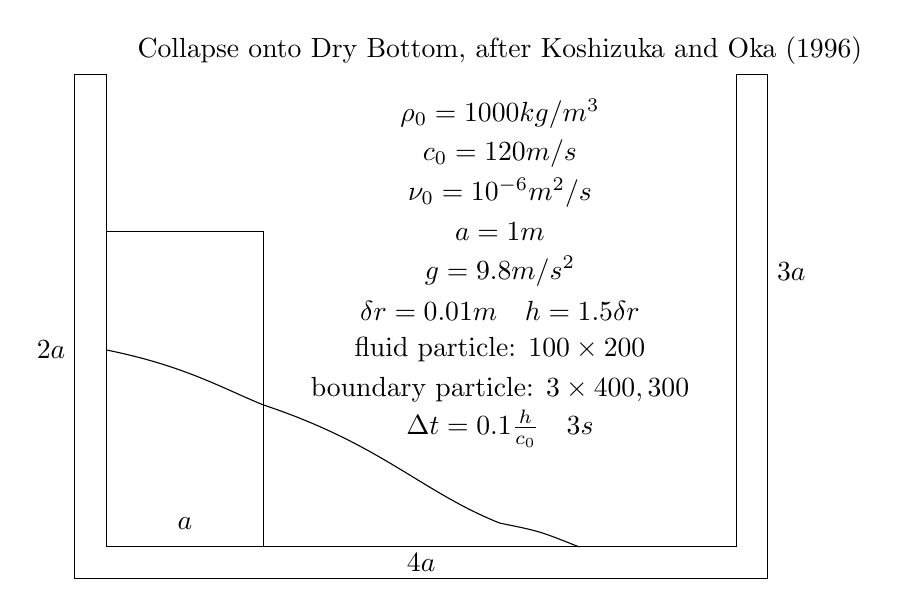
\begin{tikzpicture}
            \draw[-] (0,6)--(0,0)--(8,0)--(8,6);
            \draw[-] (0,6)--(-0.4,6)--(-0.4,-0.4)--(8.4,-0.4)--(8.4,6)--(8,6);
            \draw[-] (0,4)--(2,4)--(2,0);
            
            % arbitrary fluid surface at some time
            \draw (0,2.5) .. controls (1,2.3) and (1.5,2.0) .. (2,1.8) .. controls (3.5,1.3) and (4,0.7) .. (5,0.3) .. controls (5.5,0.2) .. (6,0);
            
            \node at (1,0.3) {$a$};
            \node at (4, -0.2) {$4a$};
            \node at (-0.7, 2.5) {$2a$};
            \node at (8.7, 3.5) {$3a$};

            \node at (5, 6.3) {Collapse onto Dry Bottom, after Koshizuka and Oka (1996)};
            \node at (5, 5.5) {$\rho_0=1000kg/m^3$};
            \node at (5, 5) {$c_0=120m/s$};
            \node at (5, 4.5) {$\nu_0=10^{-6}m^2/s$};
            \node at (5, 4) {$a=1m$};
            \node at (5, 3.5) {$g=9.8m/s^2$};
            \node at (5, 3) {$\delta r=0.01m\quad h=1.5\delta r$};
            \node at (5, 2.5) {fluid particle: $100\times 200$};
            \node at (5, 2) {boundary particle: $3\times 400,300$};
            \node at (5, 1.5) {$\Delta t=0.1\frac{h}{c_0}\quad 3s$};
        \end{tikzpicture}
    \end{figure}
\end{frame}

\subsection{踩的第一个坑:似是而非的结果}

\begin{frame}
    \frametitle{\subsecname}
    如下图,
    见 WaterWallDemo.mp4 。
    一开始我以为是对的,但再细看之下,
    发现壁面内粒子还是发生了穿透,
    只是我加的墙体粒子比较厚,未穿出。
    比如139步的右下角,就有粒子嵌入墙壁。
    \begin{figure}[H]
        \centering
        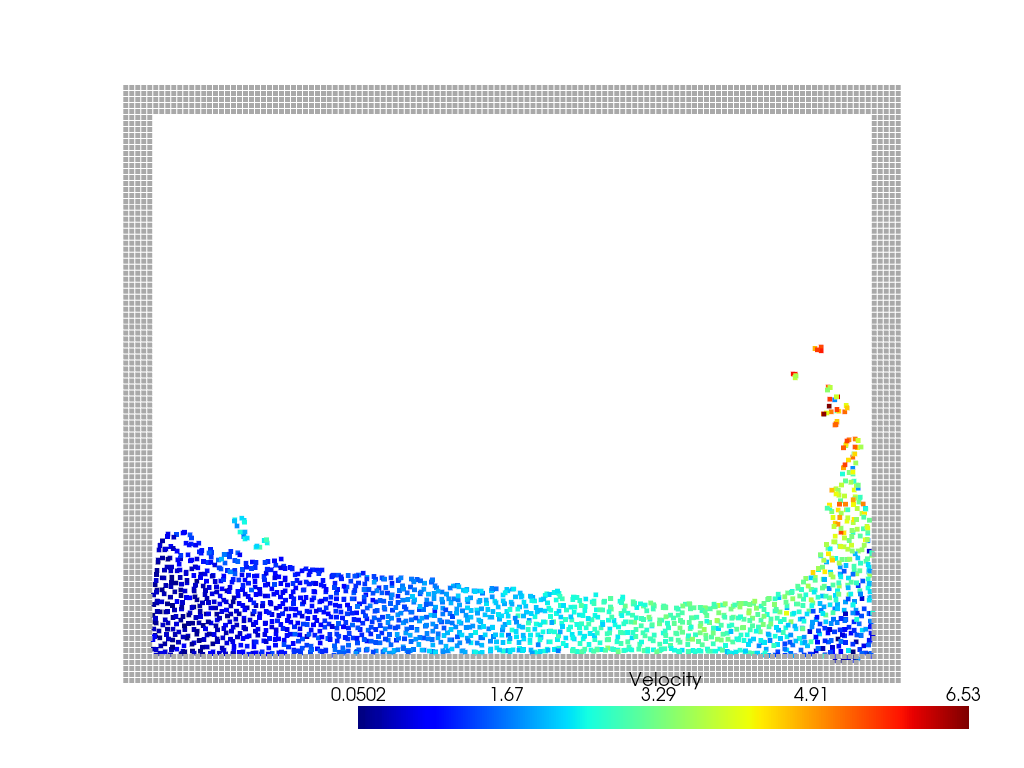
\includegraphics[width=0.7\textwidth]{images/first_trial_139.png}
    \end{figure}
\end{frame}

\subsection{踩的第二个坑:壁面的处理}

\begin{frame}
    \frametitle{\subsecname}
    然后我排查了一下程序,
    发现是在程序内壁面力没有乘 $\frac{1}{h}$ 系数。
    改完后会发现水体发生了异常的迸溅和分离,
    尤其是顶层水体像是受到了壁面异常的拍击,
    临近边界的水体有明显的异常加速,与文献不符。
    \begin{figure}[H]
        \centering
        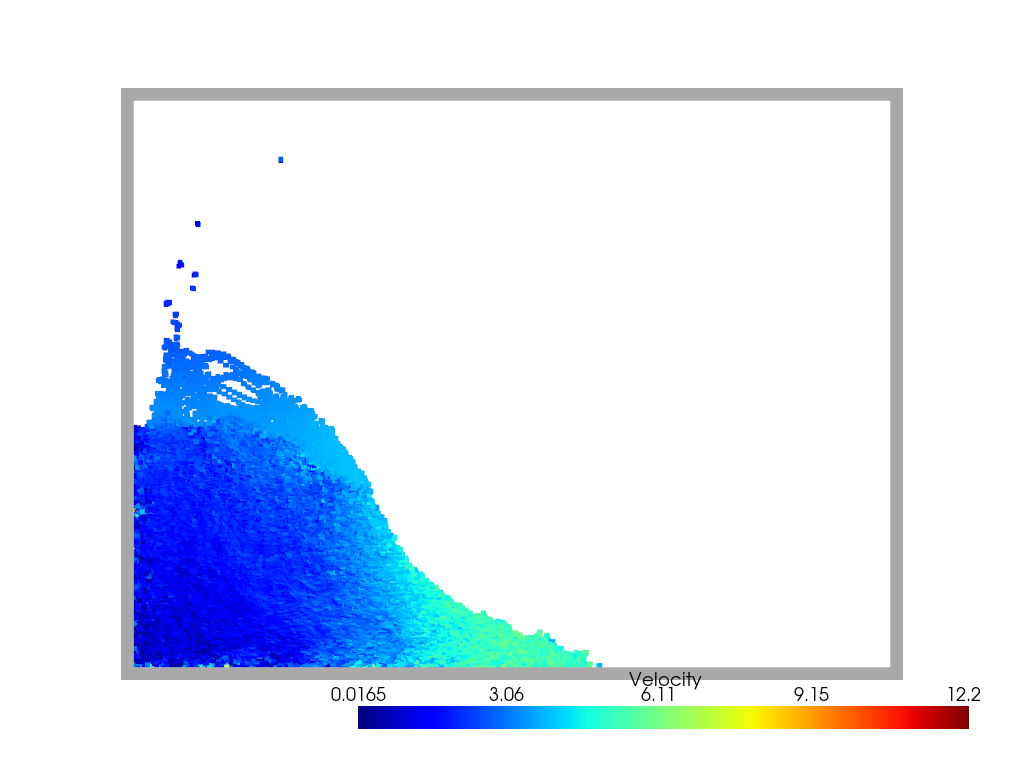
\includegraphics[width=0.7\textwidth]{images/second_trial_316.png}
    \end{figure}
\end{frame}

\begin{frame}
    \frametitle{\subsecname}
    于是我回过去推导壁面力计算公式,
    就推导出了壁面力 $f\sim 0.1k^2 n$ 的结论,
    于是怀疑可能是计算尺度的问题,
    离散化粒子太多可反而会导致计算结果不准确。
    debug 了将近一周,试了很多 $c$ 和 $h$ 以及 $dt$ 的组合。
    一无所获,程序结构还被改得很乱。
    不过这周一在看云图的过程中,
    我发现一个有趣的现象,
    下面是两张初始情况下的压强云图:
    \begin{figure}[H]
        \centering
        \subfigure[step 4]{
            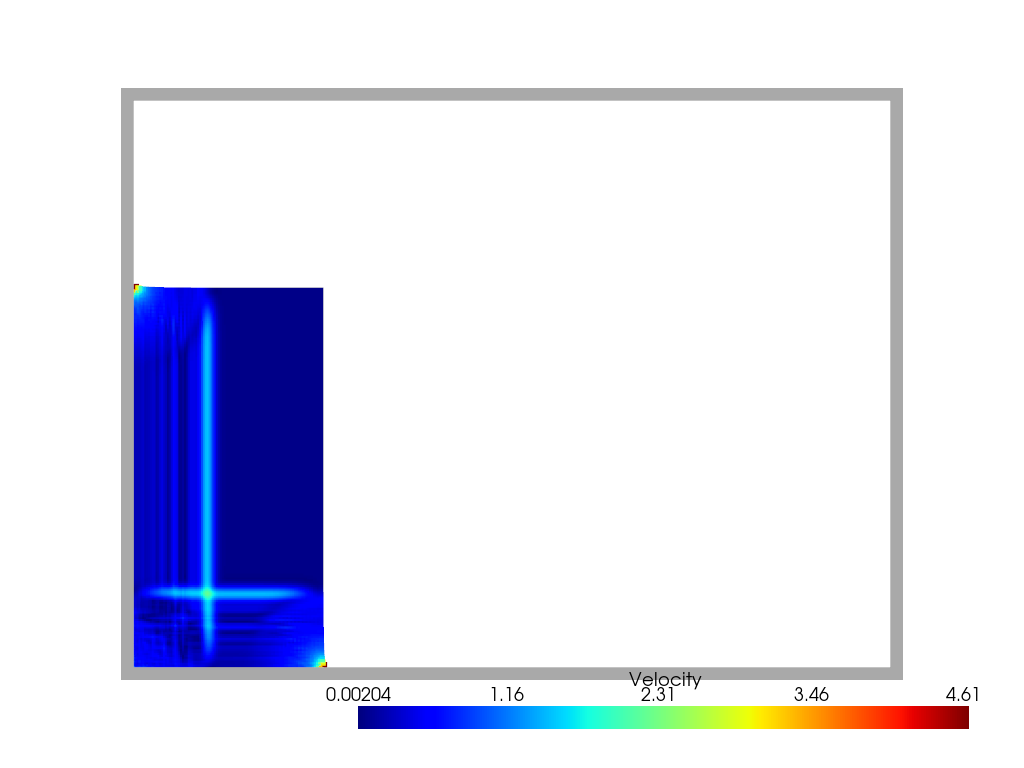
\includegraphics[width=0.45\textwidth]{images/second_trial_4.png}
        }
        \subfigure[step 6]{
            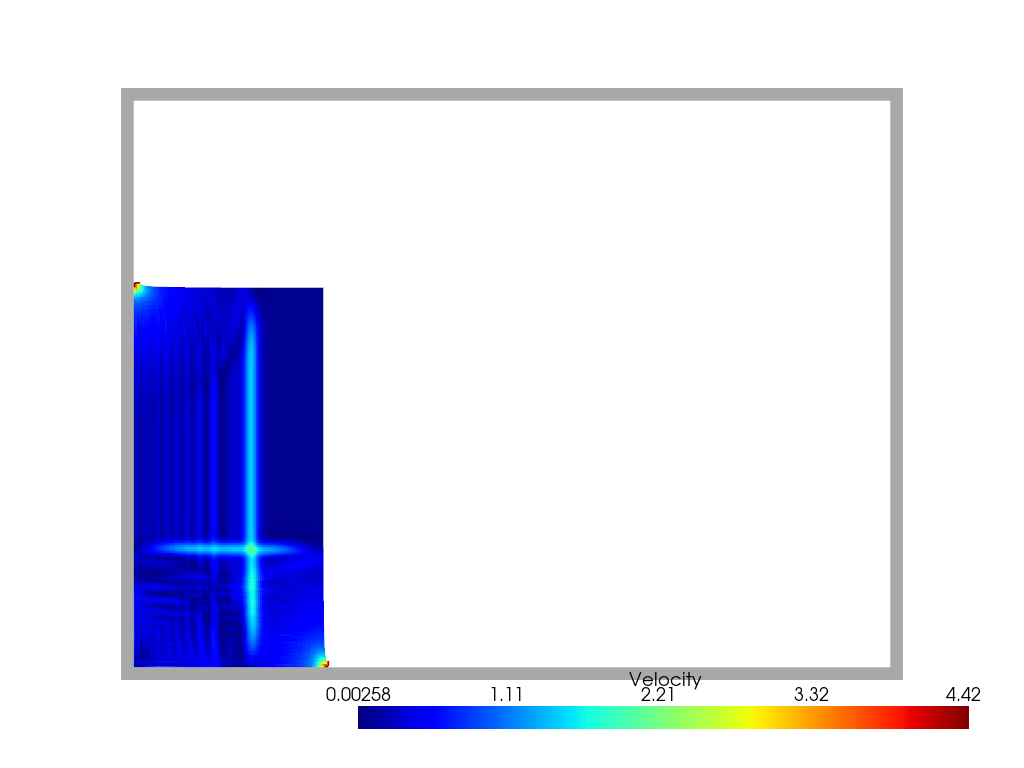
\includegraphics[width=0.45\textwidth]{images/second_trial_6.png}
        }
    \end{figure}
\end{frame}

\begin{frame}
    \frametitle{\subsecname}
    很显然的是,
    压强云图显示在初始时有一个扰动从左上角向右上角传播,
    并且同时,液体左上角开始发生崩坏,
    进而发生第一张图中的异常迸溅。
    会引起压强发生异常的水体内传播的扰动一定来源于边界力,
    于是我怀疑可能是初始时的边界给定有问题。
    \begin{figure}[H]
        \centering
        \subfigure[step 4]{
            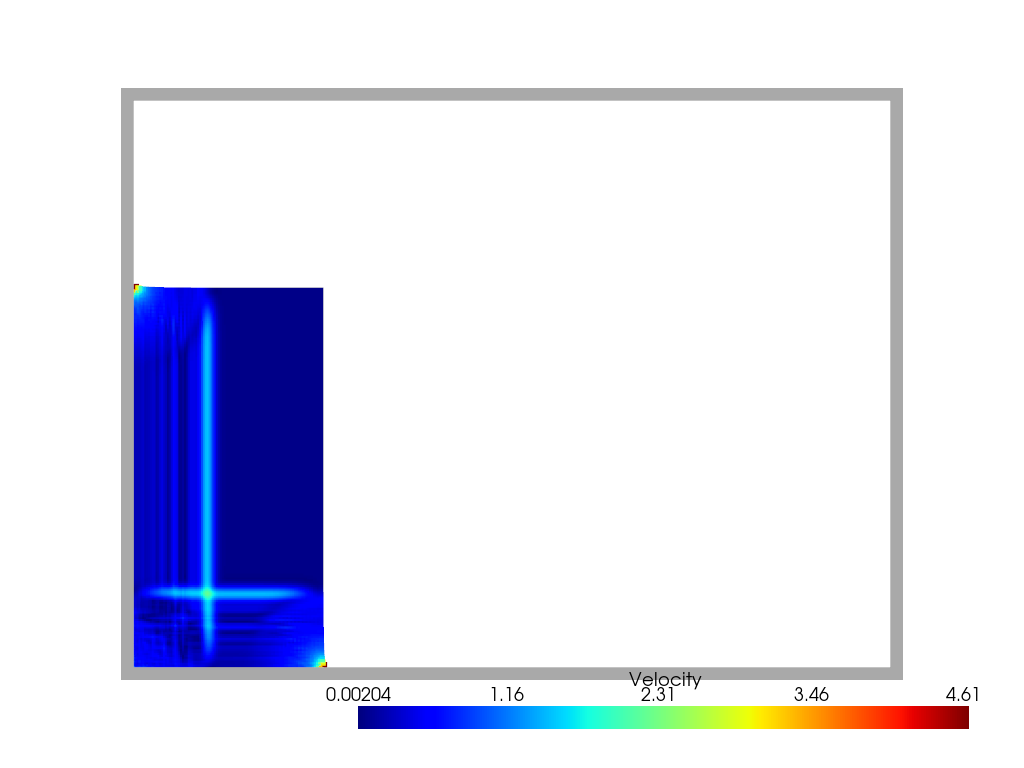
\includegraphics[width=0.45\textwidth]{images/second_trial_4.png}
        }
        \subfigure[step 6]{
            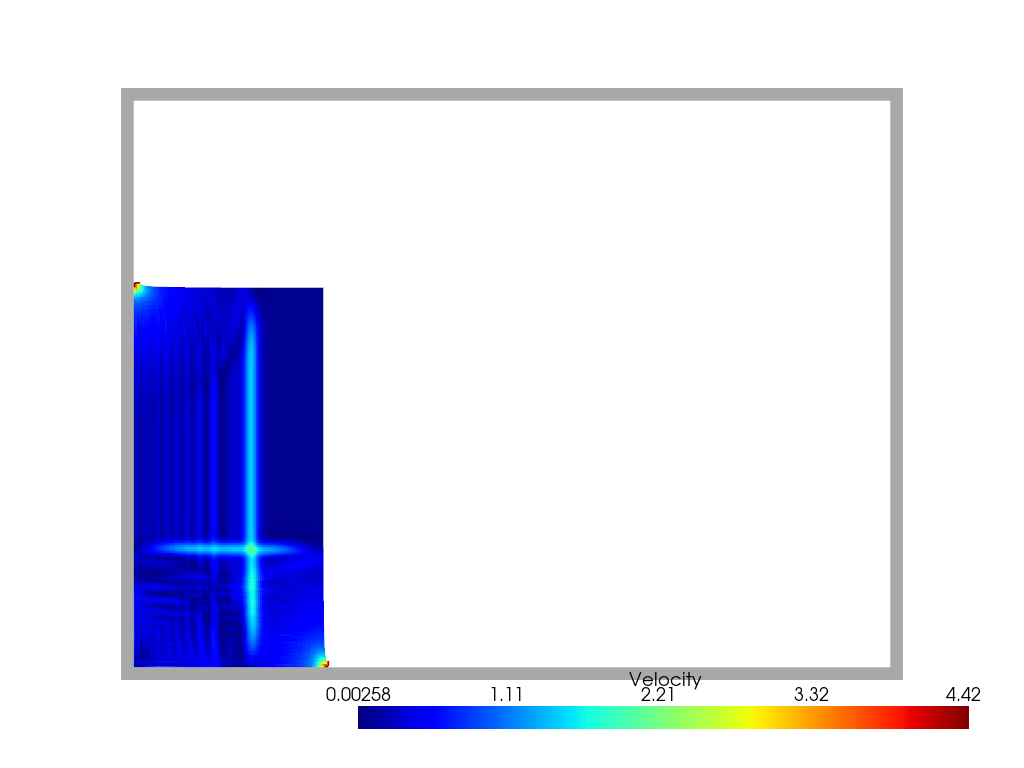
\includegraphics[width=0.45\textwidth]{images/second_trial_6.png}
        }
    \end{figure}
\end{frame}

\begin{frame}
    \frametitle{\subsecname}
    \begin{equation}
        P(\psi)=0.01\frac{1}{h}c_i^2
        \frac{1}{\sqrt{\frac{\psi}{2h}}}
        \left(1-\frac{\psi}{2h}\right)
    \end{equation}
    于是我怀疑初始边界设定不对。
    我在初始设定粒子位置时,
    是以 $dr$ 为间隔均匀分布的,
    而 $dr<h$ ,也就是初始时粒子间距小于 $h$ ,
    会有一个初始的本不该存在的初始压力项,
    而且如前所述,这项压力会给水体一个本不该存在的极大的初始扰动。
    这会让水体获得不该存在的动量,从左上角和右下角甚至水体内部崩坏。
    虽然在 SPHysics 和河海大学徐德龙教授书中公式是一致的,
    但我开始怀疑这个公式的正确性。
    \begin{figure}[H]
        \centering
        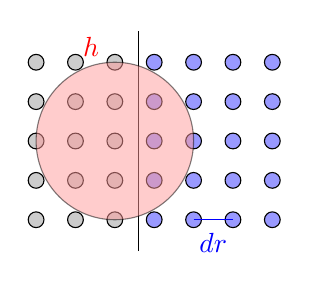
\begin{tikzpicture}
            % fluid particle
            \foreach \x in {0,1,2,3}
            \foreach \y in {0,1,2,3,4}
            \filldraw[fill=blue!40!white, draw=black] (0.5*\x,0.5*\y) circle (0.1);
            \draw[-] (-0.2,-0.4) -- (-0.2,2.4);
            % boundary particle
            \foreach \x in {-3,-2,-1}
            \foreach \y in {0,1,2,3,4}
            \filldraw[fill=gray!40!white, draw=black] (0.5*\x,0.5*\y) circle (0.1);
            
            \filldraw[fill=red!40!white, draw=black,opacity=0.5] (-0.5,0.5*2) circle (1.);

            \node[red] at (-0.8,2.2) {$h$};

            \draw[-,blue] (0.5,0) -- (1,0);
            \node[blue] at (0.75,-0.3) {$dr$};
        \end{tikzpicture}
    \end{figure}
\end{frame}

\begin{frame}
    \frametitle{\subsecname}
    鉴于 SPHysics 和徐德龙都说他们借鉴了 Rogers 在2005年的文章,
    我又去看了一下 Rogers 的文章,
    发现和 SPHysics 和徐德龙的公式完全一样,除了 $20u_{\perp}\to 40u_{\perp}$ 。
    我尝试了 Rogers 的公式,但水体崩坏的更离谱了。
    另外我还发现让 $h/dr$ 更大也会明显地让水体崩坏加剧。
    本来我以为是别的地方出了问题,
    但周二突发奇想去看了看 Rogers 引用的 Monaghan 的文章,
    发现似乎从 Rogers 开始,
    后面引用的文章全写错符号引起误解了。
    首先是沿壁面的系数 $\cos \frac{2\pi\xi}{b}$ 这项应为 $\cos \frac{\pi\xi}{b}$:
    \begin{figure}[H]
        \centering
        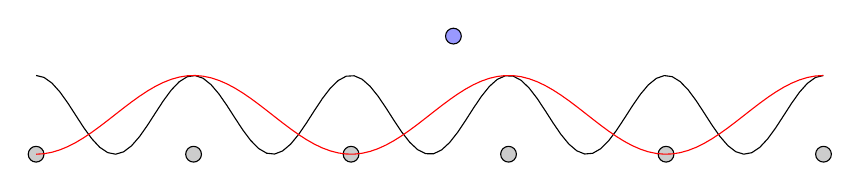
\begin{tikzpicture}
            \foreach \x in {-3,-2,-1,0,1,2}
            \filldraw[fill=gray!40!white, draw=black] (2*\x,0) circle (0.1);
            % plot cos 2pi x
            \draw[domain=-3:2,samples=100] plot (\x*2,{0.5+0.5*cos(360*\x)});
            % plot cos pi x
            \draw[domain=-3:2,samples=100,red] plot (\x*2,{0.5+0.5*cos(180*\x)});
            
            % fluid particle
            \filldraw[fill=blue!40!white, draw=black] (-0.7,1.5) circle (0.1);
        \end{tikzpicture}
    \end{figure}
\end{frame}

\begin{frame}
    \frametitle{\subsecname}
    \begin{figure}[H]
        \centering
        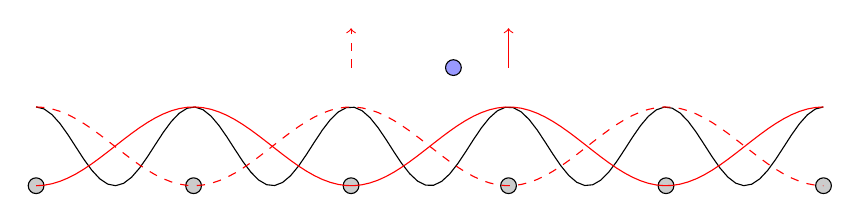
\begin{tikzpicture}
            \foreach \x in {-3,-2,-1,0,1,2}
            \filldraw[fill=gray!40!white, draw=black] (2*\x,0) circle (0.1);
            % plot cos 2pi x
            \draw[domain=-3:2,samples=100] plot (\x*2,{0.5+0.5*cos(360*\x)});
            % plot cos pi x
            \draw[domain=-3:2,samples=100,red] plot (\x*2,{0.5+0.5*cos(180*\x)});
            \draw[domain=-3:2,samples=100,red,dashed] plot (\x*2,{0.5+0.5*cos(180*(\x-1)});
            % fluid particle
            \filldraw[fill=blue!40!white, draw=black] (-0.7,1.5) circle (0.1);
            
            \draw[->,red] (0,1.5)--(0,2.0);
            \draw[->,red,dashed] (-2,1.5)--(-2,2.0);
        \end{tikzpicture}
    \end{figure}
    如上图所示,
    黑线为 $\frac{1}{2}\left(1+\cos \frac{2\pi\xi}{b}\right)$ ,
    红线为 $\frac{1}{2}\left(1+\cos \frac{\pi\xi}{b}\right)$ ,
    对于陷在两壁面粒子间的流体粒子而言,
    会受两个相邻壁面粒子的联合作用。
    对于 Monaghan 的公式,
    红色的 $\cos$ 起到叠加恒等的效果,
    而黑色的徐德龙和 Rogers 以及 SPHysics 的公式,
    在极端情况下(流体粒子在壁面粒子中间),
    两者叠加为 $0$ ,
    粒子会直接穿透壁面,不受阻碍。
\end{frame}

\begin{frame}
    \frametitle{\subsecname}
    其次是 $h$ 和 $b$ 符号的问题。
    Monaghan 原文中提到:
    where $R( y)$ is designed to fall to zero within a few particle spacings of the wall. 
    In the simulations described here, $R( y)$ is defined in terms of $q = y/(2\delta p)$ 
    (where $\delta p$ is the initial particle spacing) by the rule.
    If $q<1$ then:
    \begin{equation}
        R(y)=A\frac{1}{\sqrt{q}}(1-q)
    \end{equation}
    otherwise $R(y)=0$.
    The form of $R( y)$ is not crucial but the force must increase as $q$ decreases.
    说白了,壁面效应的作用范围不超出两倍的初始粒子间距。
    而不是光滑核半径。
    并且 $A$ 的选取也比较随意(因为这个边界叫 conpulsive boundary)。
    于是为了避免初始时的异常扰动,
    我调整了 $q/2h\to q/b$
    并进行了仿真。
    设置如前面所述,
    总共 $100\times 200$ 个流体粒子,
    $3\times (400+3+3+300\times 2)$ 个壁面粒子。
    仿真时间 $3s$ ,仿真总步数 24 万步。
\end{frame}

\subsection{目前该算例最好的计算结果以及文献对比}

\begin{frame}
    \frametitle{\subsecname}

    240.0k/240.0k [03:11:28<00:00, 21it/s]
    11489.689665 seconds (225.90 G allocations: 25.249 TiB, 17.03\% gc time, 0.03\% compilation time)

    这个程序运行了大约 11489.689665 秒(约等于 3 小时 11 分钟 28 秒),在这个过程中,它进行了大约 225.90 G(G表示十亿)次内存分配,总共分配了大约 25.249 TiB(TiB 是 Tebibyte,1 TiB 等于 1024 GiB)的内存。其中,17.03\% 的时间被用于垃圾回收(gc),0.03\% 的时间被用于编译。
    见 CollapseDry.mp4 。
\end{frame}

\begin{frame}
    \frametitle{\subsecname 0.5s}
    \begin{figure}[H]
        \centering
        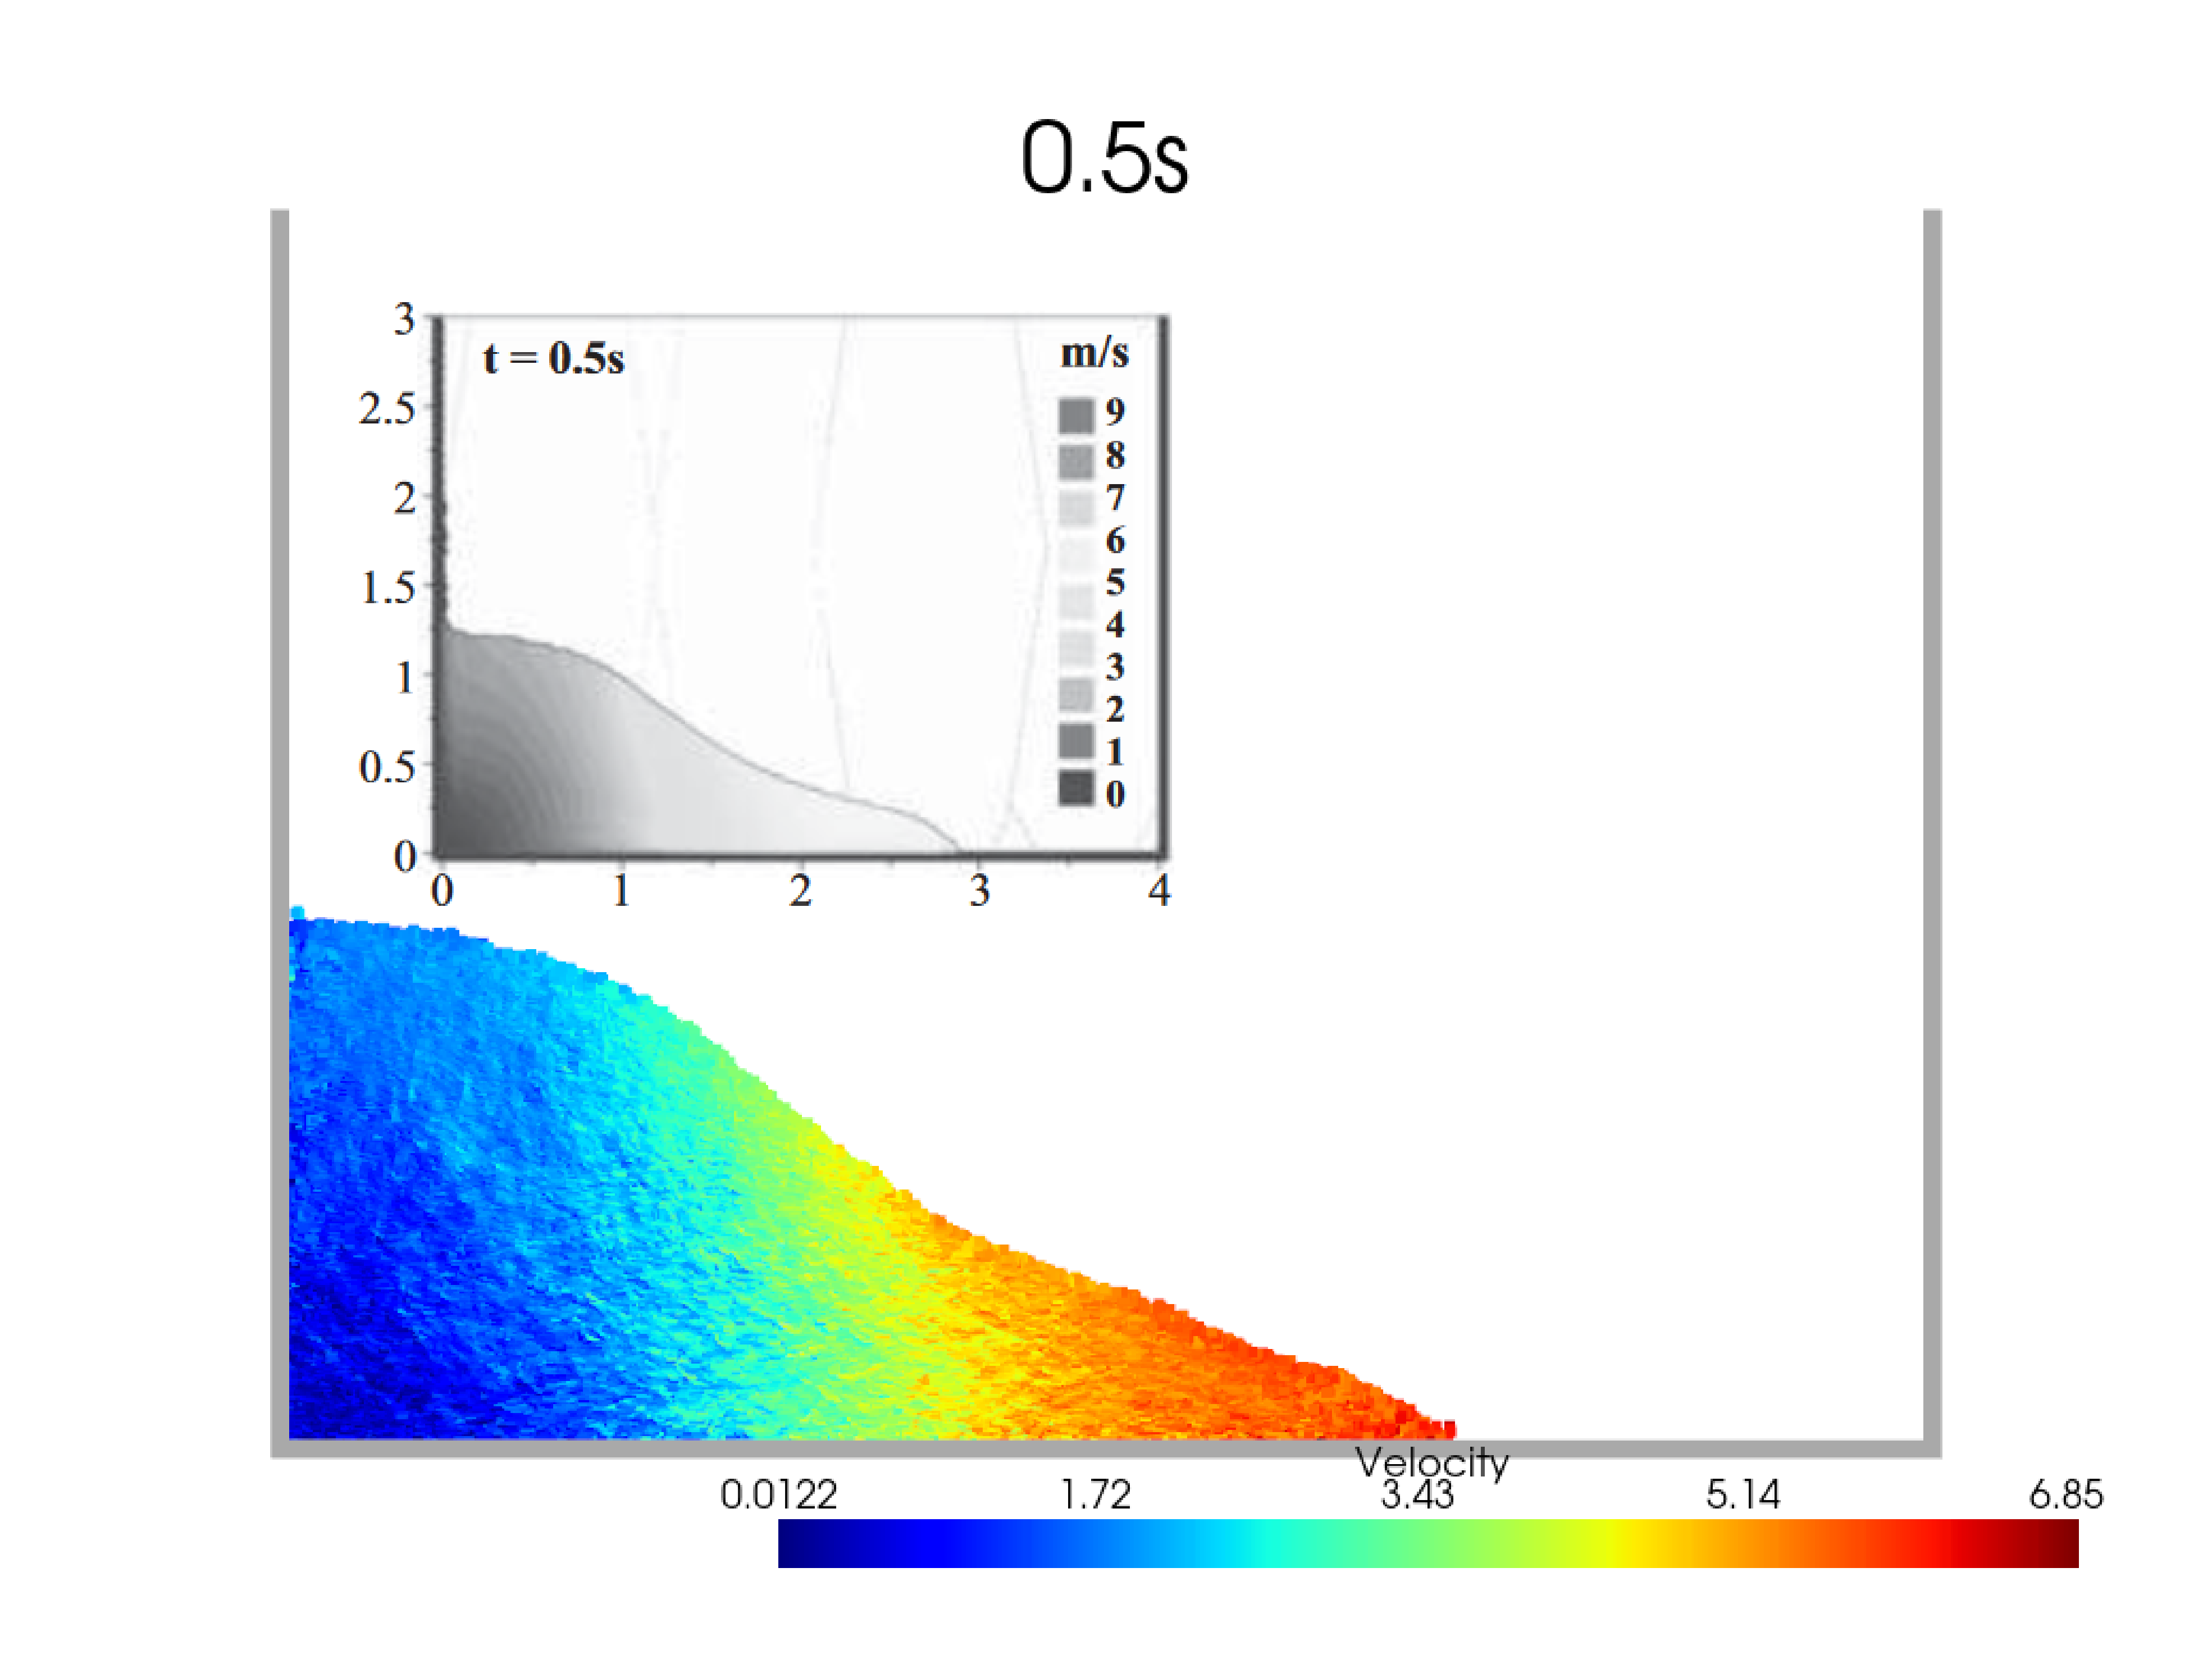
\includegraphics[width=0.9\textwidth]{images/collapse_dry05_combined.png}
    \end{figure}
\end{frame}

\begin{frame}
    \frametitle{\subsecname 1.1s}
    \begin{figure}[H]
        \centering
        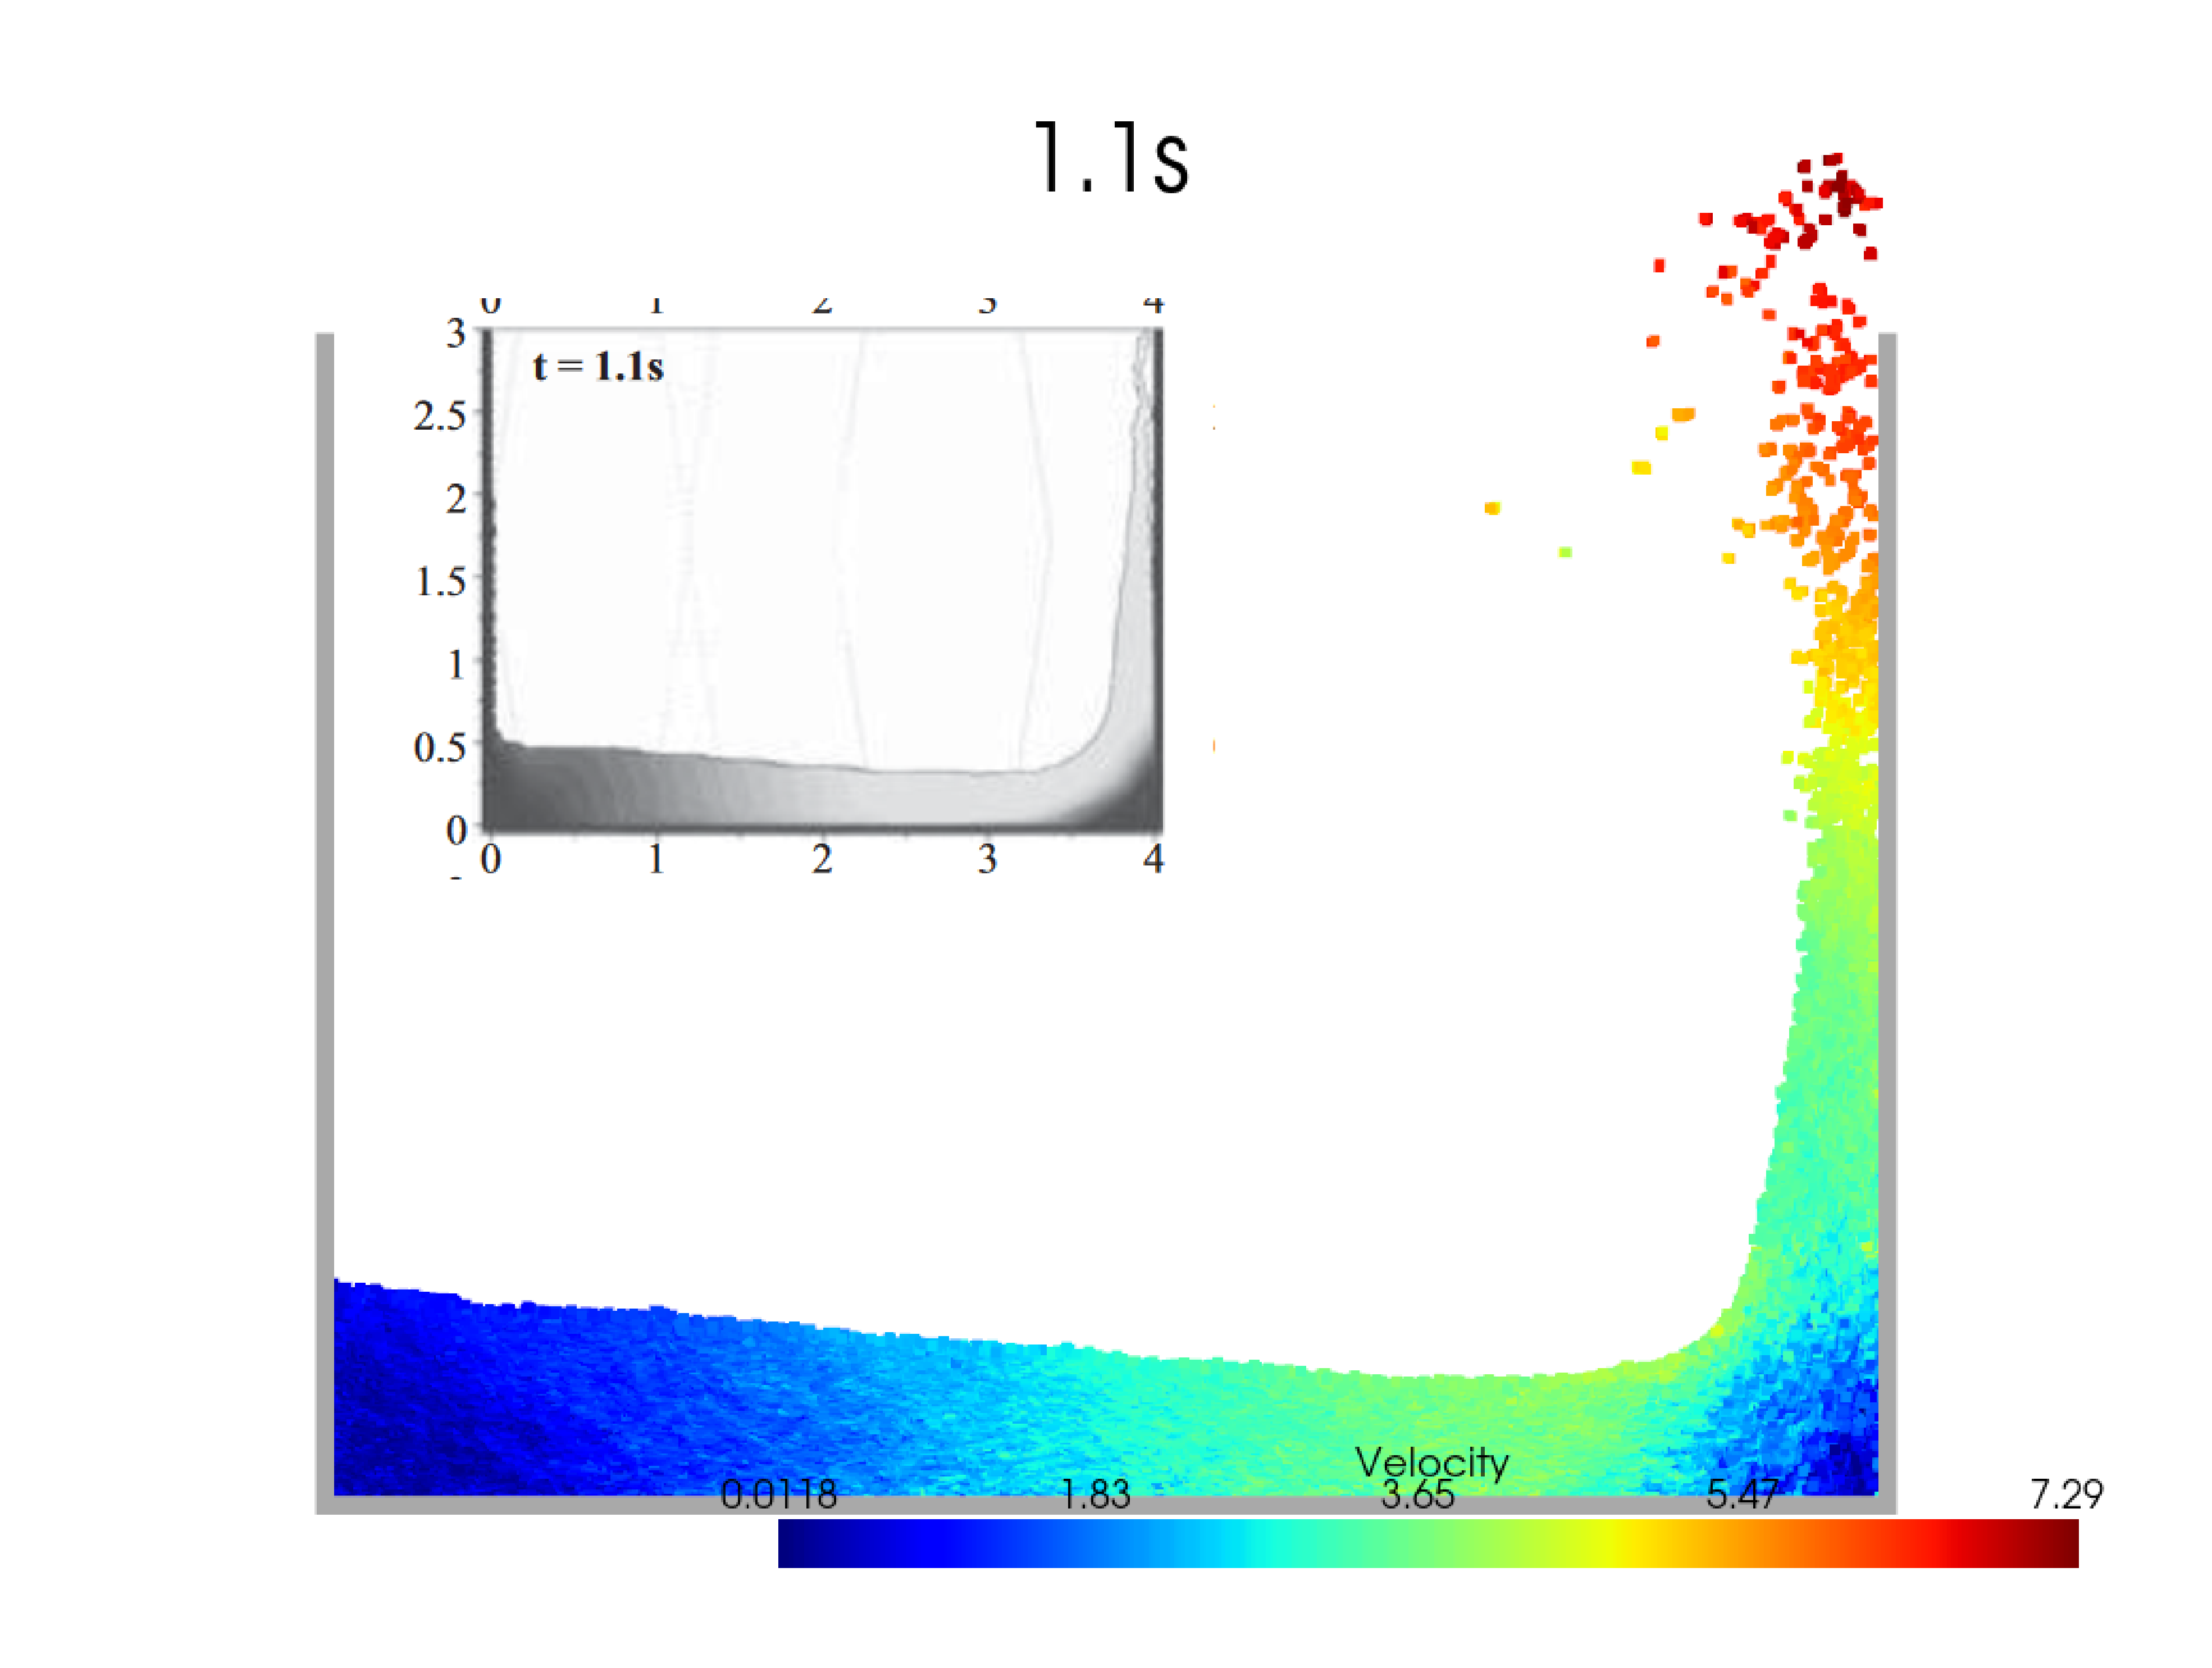
\includegraphics[width=0.9\textwidth]{images/collapse_dry11_combined.png}
    \end{figure}
\end{frame}

\begin{frame}
    \frametitle{\subsecname 1.8s}
    \begin{figure}[H]
        \centering
        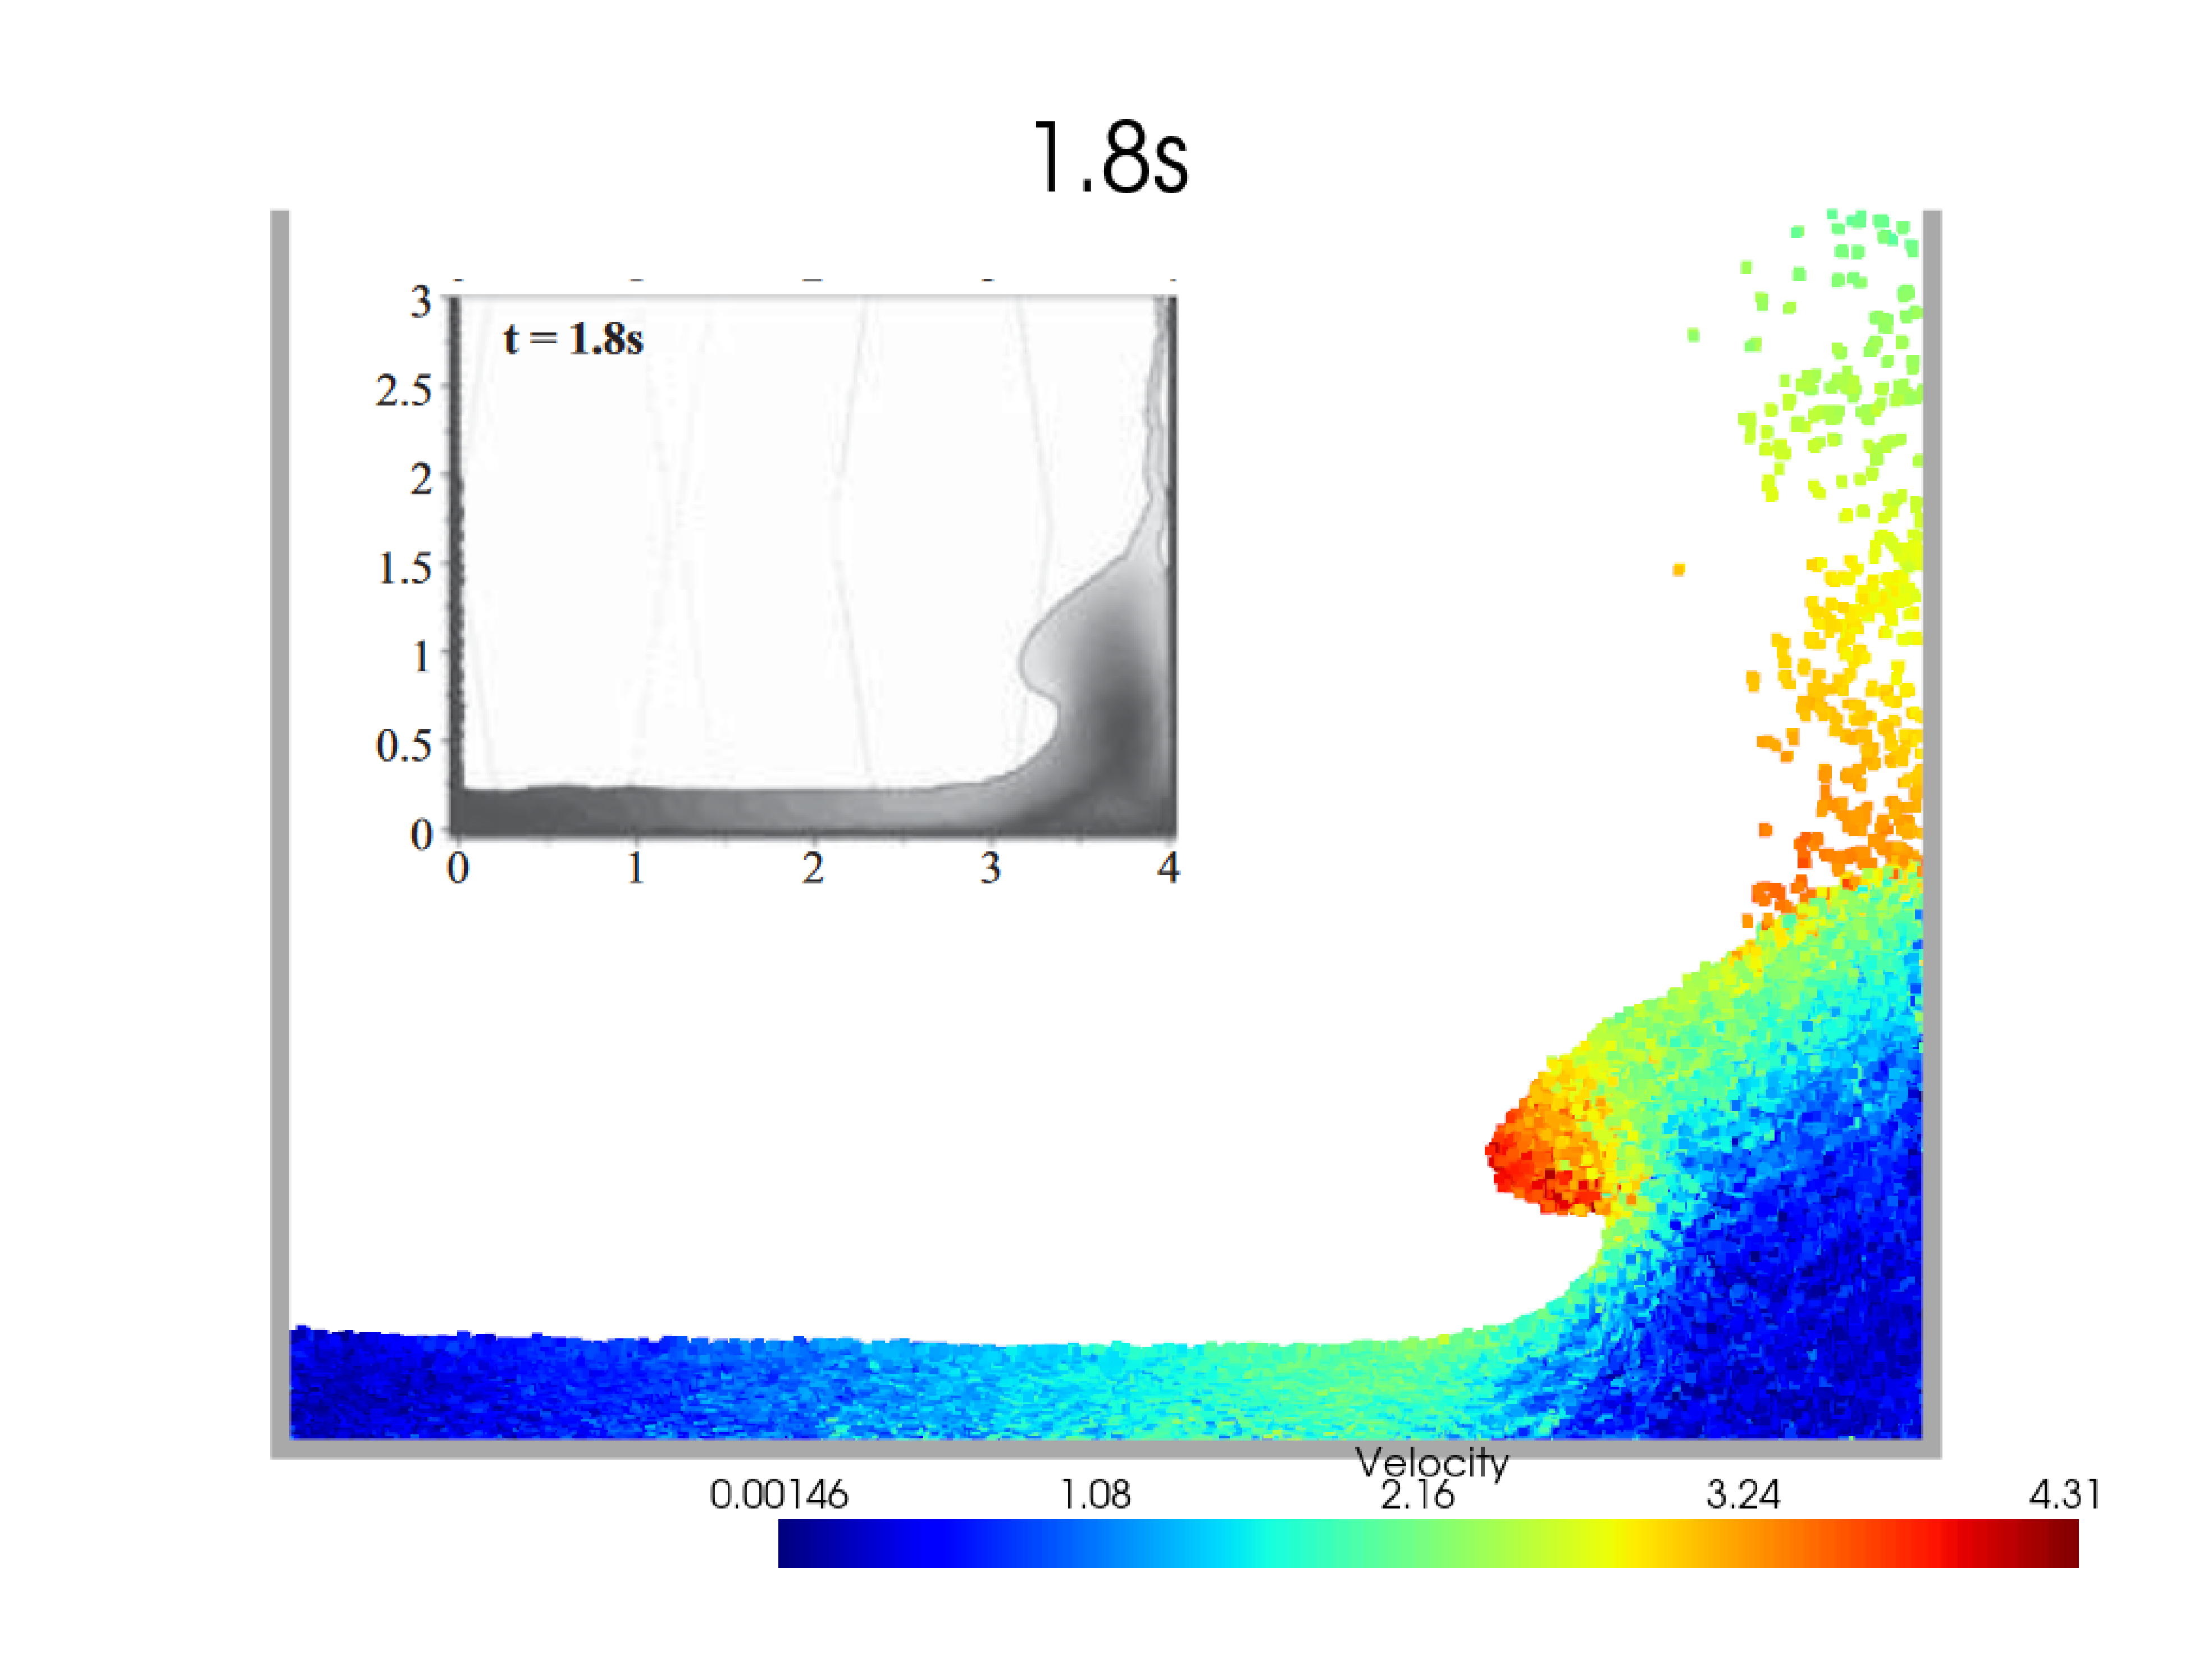
\includegraphics[width=0.9\textwidth]{images/collapse_dry18_combined.png}
    \end{figure}
\end{frame}

\begin{frame}
    \frametitle{\subsecname 2.1s}
    \begin{figure}[H]
        \centering
        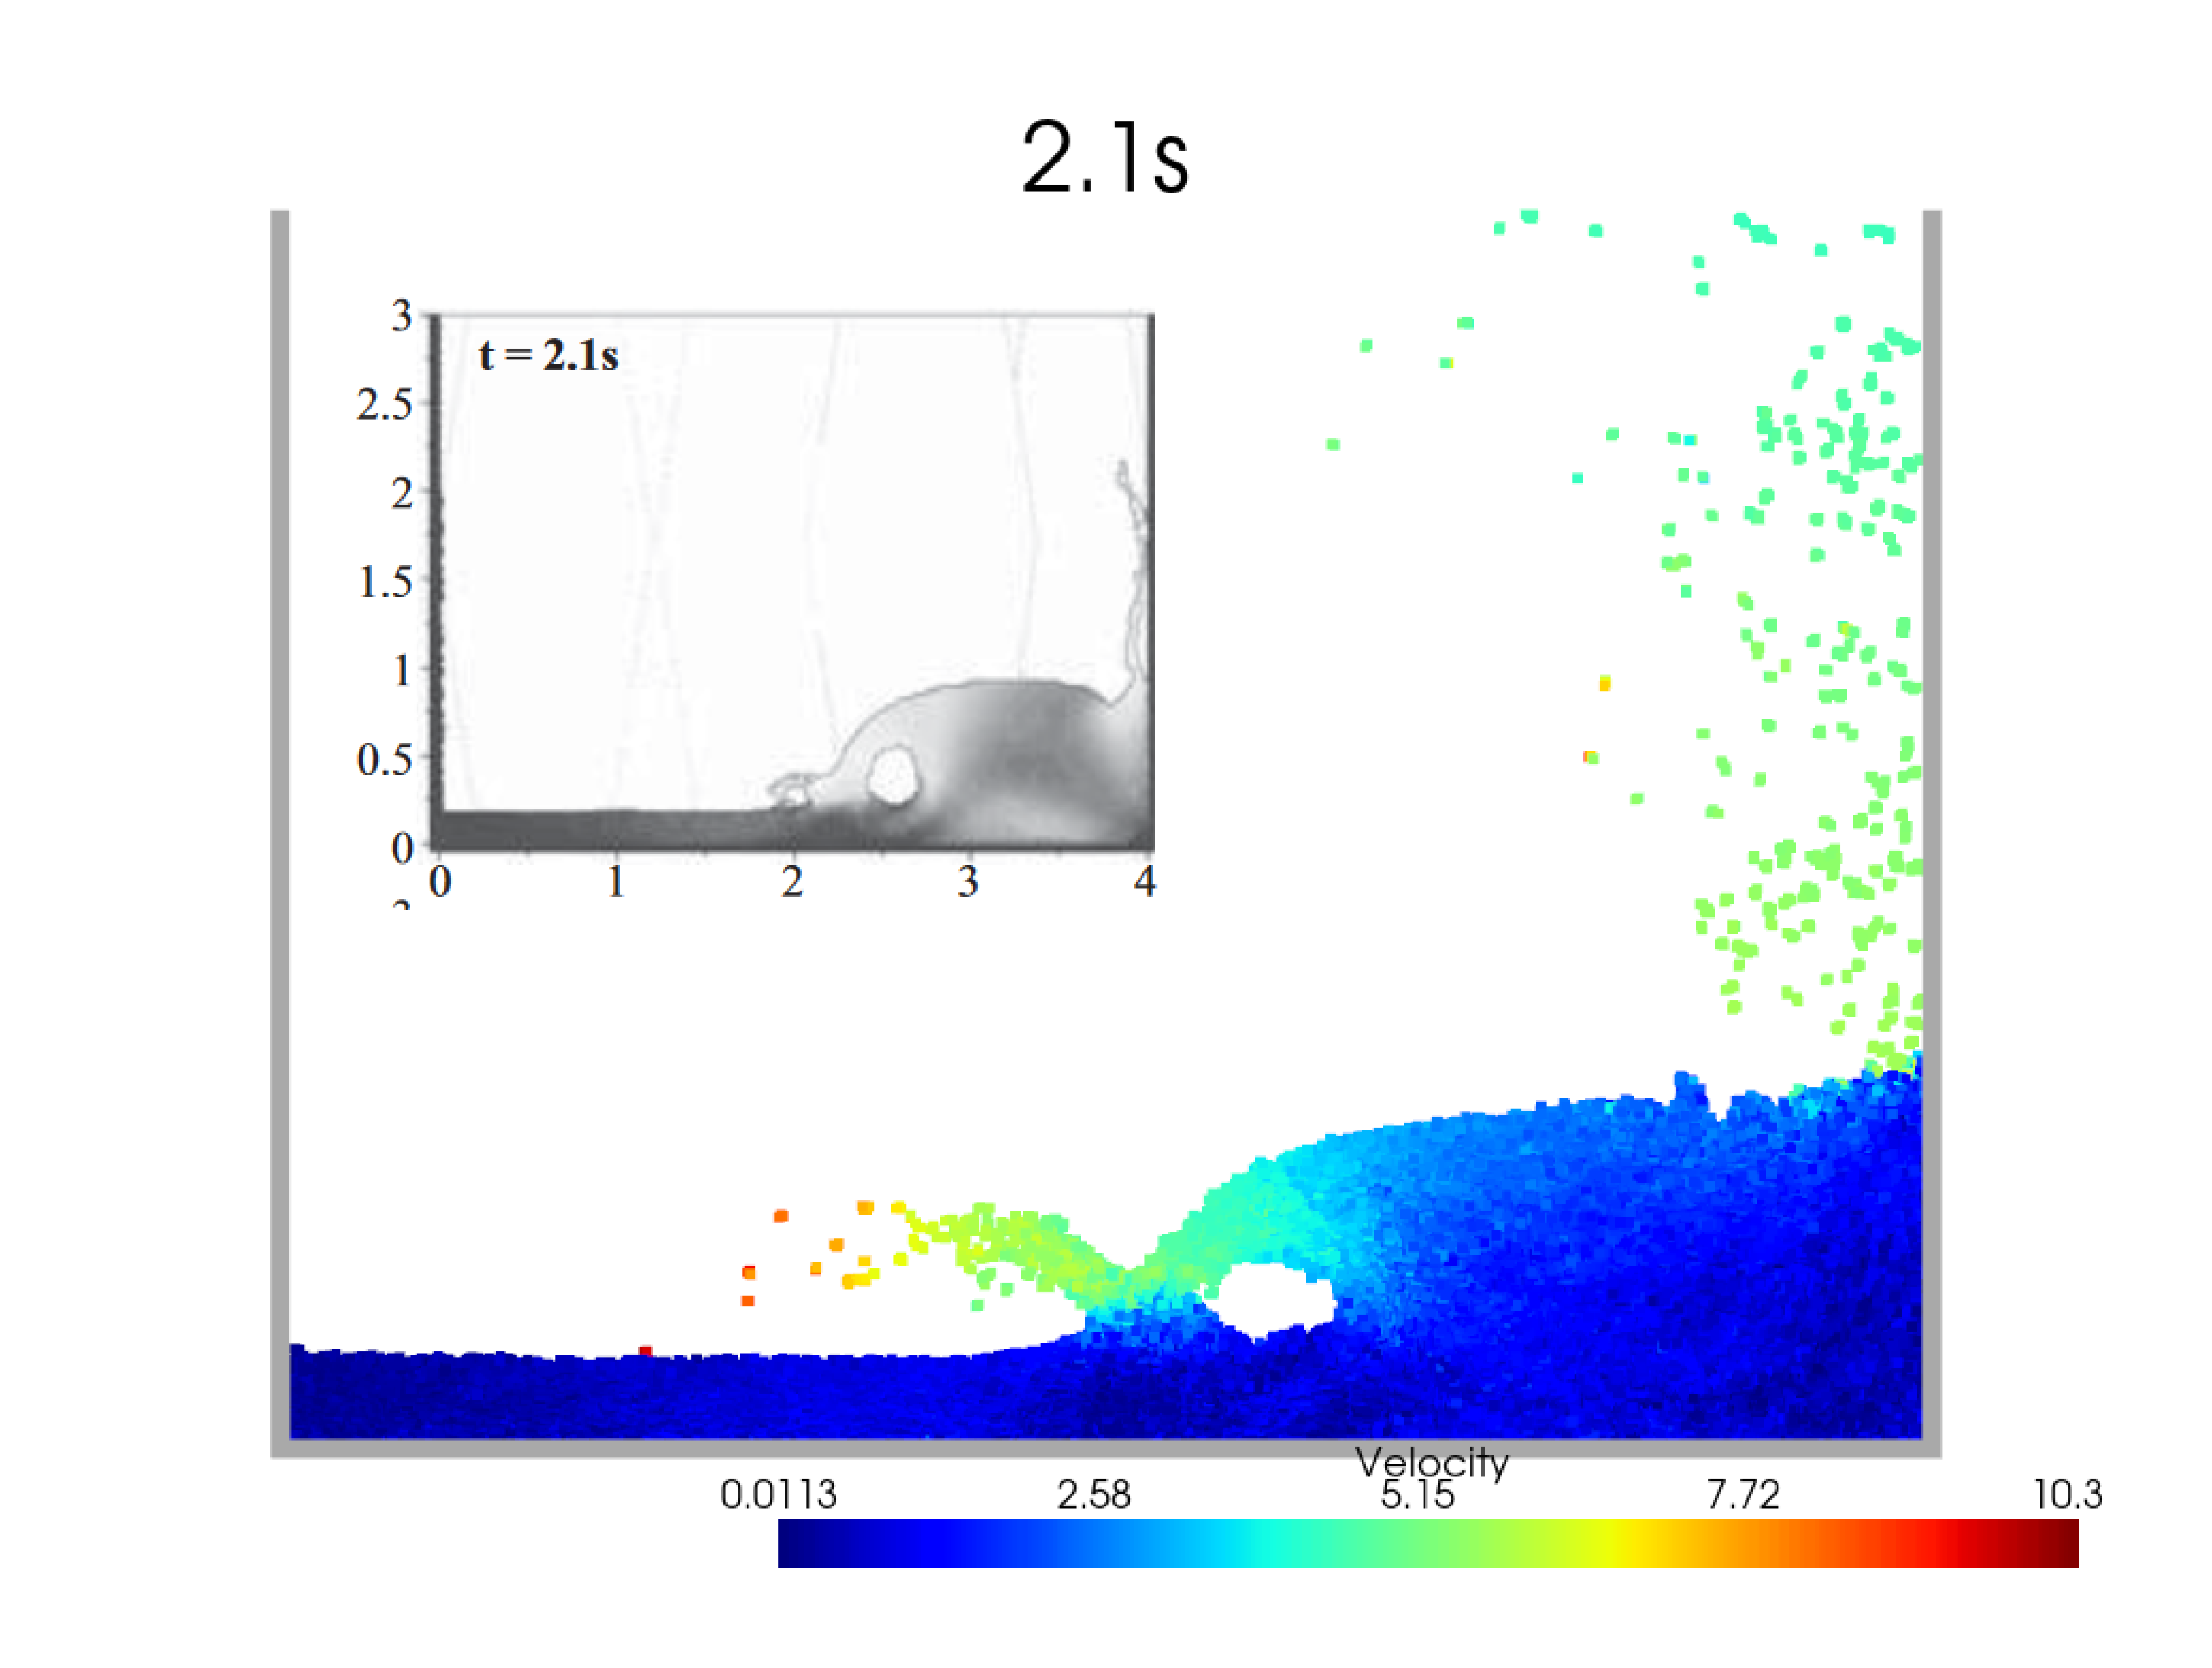
\includegraphics[width=0.9\textwidth]{images/collapse_dry21_combined.png}
    \end{figure}
\end{frame}

\begin{frame}
    \frametitle{\subsecname 2.7s}
    \begin{figure}[H]
        \centering
        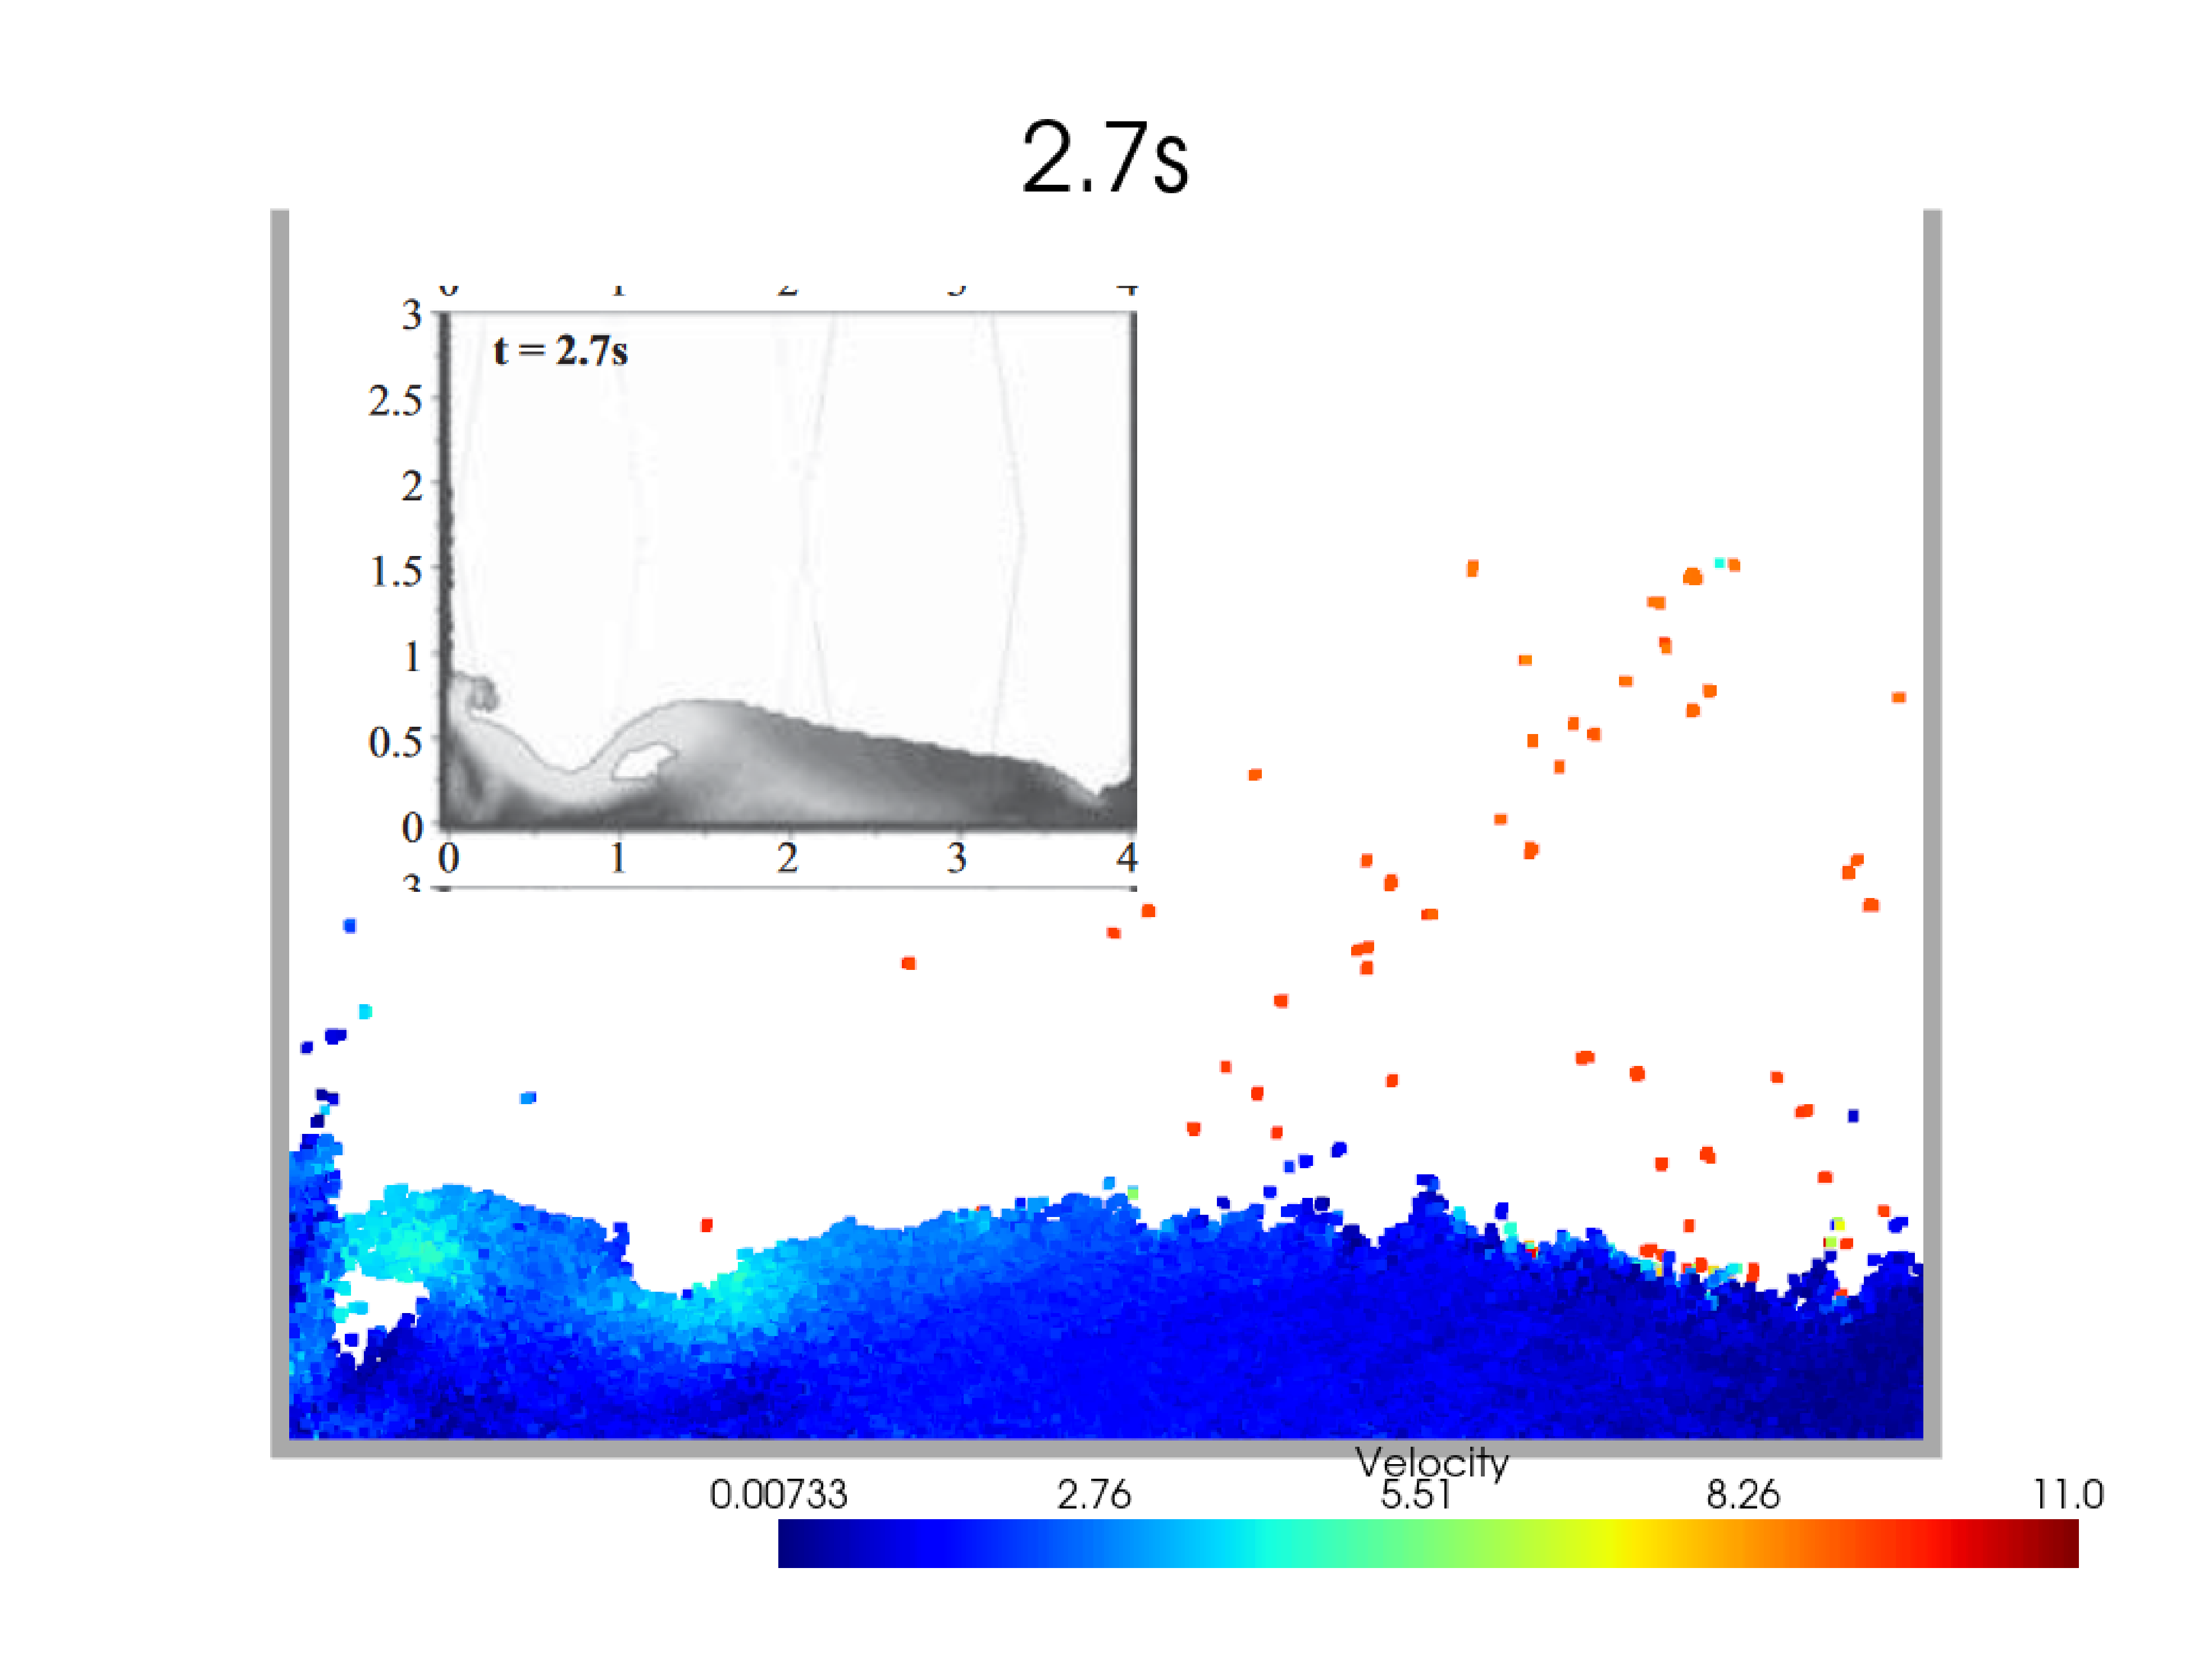
\includegraphics[width=0.9\textwidth]{images/collapse_dry27_combined.png}
    \end{figure}
\end{frame}

\begin{frame}
    \frametitle{\subsecname 2.9s}
    \begin{figure}[H]
        \centering
        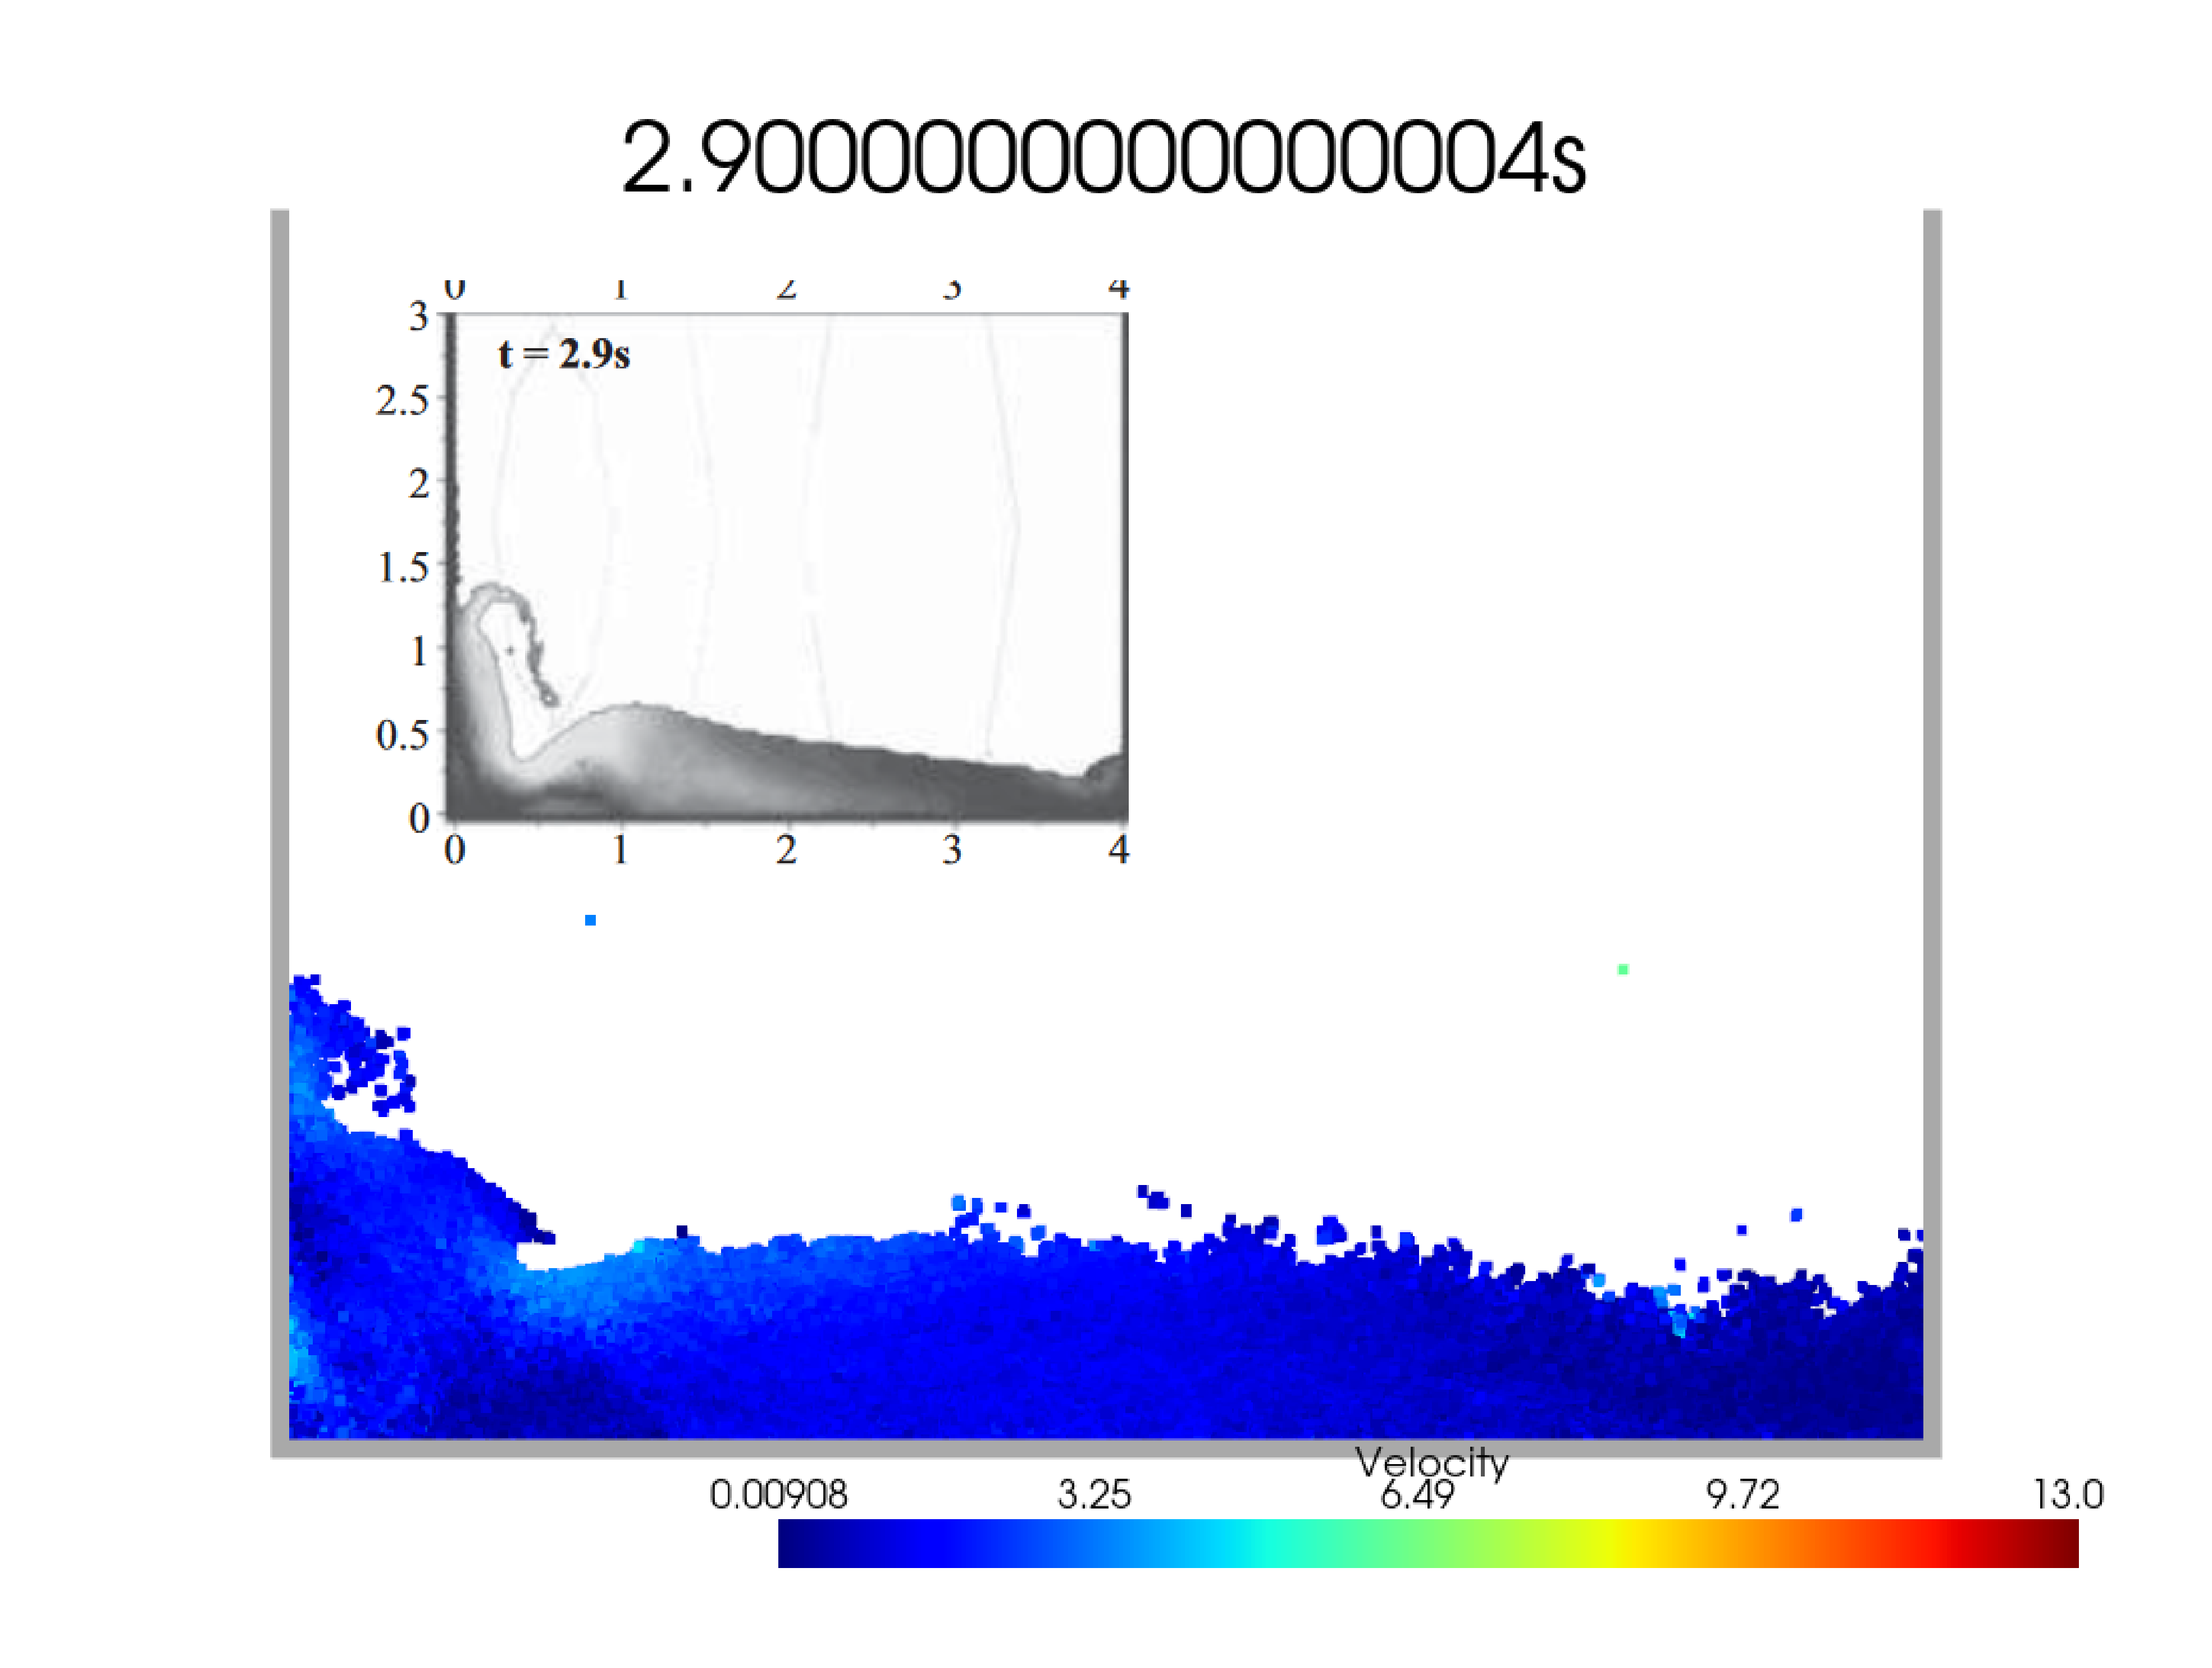
\includegraphics[width=0.9\textwidth]{images/collapse_dry29_combined.png}
    \end{figure}
\end{frame}